\documentclass[12pt, spanish]{article}

\usepackage[activeacute]{babel}
\usepackage[utf8x]{inputenc}
\usepackage[T1]{fontenc}
\spanishdecimal{.}

\usepackage{amsmath, amsthm}
\usepackage{amssymb}
\usepackage{booktabs}

\usepackage{graphicx}
\usepackage{subfigure}
\usepackage{natbib}
\usepackage[hidelinks]{hyperref}
\usepackage{enumitem}

\newtheoremstyle{problemstyle}  % <name>
        {3pt}                                               % <space above>
        {3pt}                                               % <space below>
        {\normalfont}                               % <body font>
        {}                                                  % <indent amount}
        {\bfseries\itshape}                 % <theorem head font>
        {\normalfont\bfseries:}         % <punctuation after theorem head>
        {.5em}                                          % <space after theorem head>
        {}                                                  % <theorem head spec (can be left empty, meaning `normal')>
\theoremstyle{problemstyle}

\newtheorem{problem}{Problema}[section] % Comment out [section] to remove section number dependence

\newcommand\TheSolution{\textbf{Solución:}}
\newcommand\ASolution{\textbf{SolTrace:}}


\usepackage{listings}
\usepackage{color}

\definecolor{mygreen}{rgb}{0,0.6,0}
\definecolor{mygray}{rgb}{0.5,0.5,0.5}
\definecolor{mymauve}{rgb}{0.58,0,0.82}

\lstset{ 
  backgroundcolor=\color{white},
  basicstyle=\footnotesize,
  breakatwhitespace=false,
  breaklines=true,
  captionpos=b,
  commentstyle=\color{mygreen},
  deletekeywords={...},
  escapeinside={\%*}{*)},
  extendedchars=true,
  frame=single,
  keepspaces=true,
  keywordstyle=\color{red},
  language=C,
  morekeywords={*,cwd, define, sunopt, clearopticss, addoptic, opticopt, clearstages, addstage, addelement, activestage, asselement, elementopt, traceopt, trace, elementstats, write_line, open, close, save_project, cos, exp, acos, outln},
  numbers=left,
  numbersep=5pt,
  numberstyle=\tiny\color{mygray},
  rulecolor=\color{black},
  showspaces=false,
  showstringspaces=false,
  showtabs=false,
  stepnumber=2,
  stringstyle=\color{mymauve},
  tabsize=2,
  title=\lstname
}


\author{Isaías Moreno Cruz}
\title{Curso de SolTrace}

\begin{document}
\maketitle


\section{Introducción}
\label{sec:rayos}

Una forma de cálcular la irradiancia solar concentrada es la simulación de \emph{trazado de rayos}, el cual se puede llevar a cabo mediante dos métodos:

\begin{itemize}[noitemsep]
  \item El método de \emph{Monte Carlo}, basado en rayos al azar (método estadístico)
  \item El método de \emph{Convolución}, basado en la convolución de distribuciones.
\end{itemize}

El método de Monte Carlo usa rayos al azar que vienen de una superficie, y luego determina cuales de ellos llegan a una segunda superficie. La irradiancia sobre una superficie elemental es proporcional al número de impactos de rayos. En el caso de un concentrador con una reflexión, este algoritmo es usado dos veces, primero entre el Sol y la superficie reflectiva con una distribución energética correspondiente de la forma del sol, después entre la faceta del helióstato y el receptor con las leyes estadísticas del error de distribución relacionado con los defectos de las facetas. La precisión y el tiempo de cálculo aumentan con el número de rayos y la complejidad de la geometría. En el método de convolución (o cono óptico), los rayos reflejados de los espejos elementales  son considerados con un cono de error calculado por la convolución de la distribución normal Gausiana correspondiente a cada error (forma del Sol y los errores del helióstato). Una comparación sistemática muestra que se obtienen resultados muy similares con ambos métodos de trazo de rayos, aunque el Método de Monte Carlo  es más versátiles \citep{Garcia2008codes}.


\section{SolTrace}
\label{sec:soltrace}

\textbf{SolTrace} es un software que utiliza el trazado de rayos por el método de Monte Carlo, desarrollado por el \href{https://www.nrel.gov/csp/soltrace.html}{NREL}, que puede usarse para analizar y diseñar sistemas ópticos de potencia de energía solar. El cual puede ser adaptado a las principales tecnologías de conversión de energía térmica solar a electricidad y también a hornos solares. El sistema óptico esta organizado en etapas en un sistema de coordenadas globales: las etapas son secciones de la geometría óptica que exitosamente es golpeada por los rayos en su trayectoria del sol a el receptor final. Las etapas pueden ser ópticas (interacción física con los rayos) o virtuales (usadas para determinar la posición de los rayos o el mapa de flujo en cualquier parte del sistema sin interacción con él). Estas etapas estan compuestas de elementos con su propia apertura, forma, y propiedades ópticas (errores ópticos, error de especularidad, refletividad, transmitividad, y reflacción). Cada elemento esta descrito en un sistema coordinado asociado con su etapa. A diferencia de las otras herramientas, atenuación atmosférica y errores de seguimiento no se incluyen directamente pero pueden ser tomadas en cuenta, respectivamente, en la reflectivilidad del espejo o en su error de pendiente \citep{Wendelin2013soltrace}. Los resultados pueden ser mostrados y guardados como gráficas, mapas de flujo y gráficas de desempeño, además de tener una interface amigable con el usuario.


La Figura~\ref{fig:indice} muestra las etapas necesarias para relizar una simulación en SolTrace, es decir:

\begin{itemize}[noitemsep]
\item \emph{Sun Shape}
\item \emph{Optical Properties}
\item \emph{System Stages}
\item \emph{Trace Options}
\item \emph{Results}
\end{itemize}

\subsection{Forma Solar}
\label{subsec:forma}

En el apartado de la forma solar (\emph{sun shape}) podemos indicar la \textbf{dirección del vector solar} mediante \emph{coordenadas globales}, que identificaremos como $\hat s$, o al ingresar los parámetros de \emph{latitud, día y hora}.

En el caso de que nosotros ingresemos el vector solar $\hat s$, nos permite definir nuestro sistema de referencia, es decir, que $x$, $y$ y $z$ estarán referenciadas según nuestro propio interés. En este caso, y para todo el presente manual, los sistemas de referencia serán $x$ hacia el este, $y$ hacia el norte y $z$ hacia el cenit. Cuando ingresamos la latitud, el día y la hora entonces el sistema de referencia estará dado por el sistema global de SolTrace que considera $x$ hacia el oeste, $z$ hacia el norte y $y$ hacia el cenit.

Una vez que se haya indicado la dirección del vector solar hay que indicar la forma solar. La forma solar es la distribución de intensidad de los rayos solares que llegan a la siperficie de la Tierra como función de su ángulo con respecto al centro del disco solar. Esta forma no es constante en el tiempo y tampoco es independiente de la localización geográfica, ya que se ve afectada por las condiciones climáticas. Existen diferentes formas solares: el sol uniforme (\emph{pillbox}), el sol Gaussiano, y el sol real~\citep{Buie2003sunshape}. 

\begin{figure}[h!]
  \centering
  \subfigure[]{
    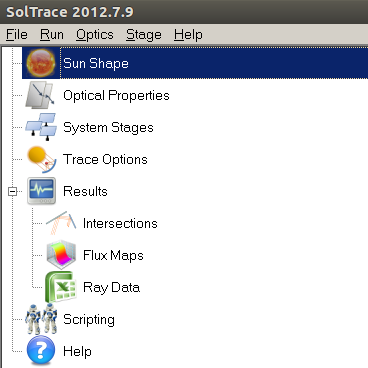
\includegraphics[width=0.315\textwidth]{figures/SolTrace}\label{fig:indice}}
  \subfigure[]{
  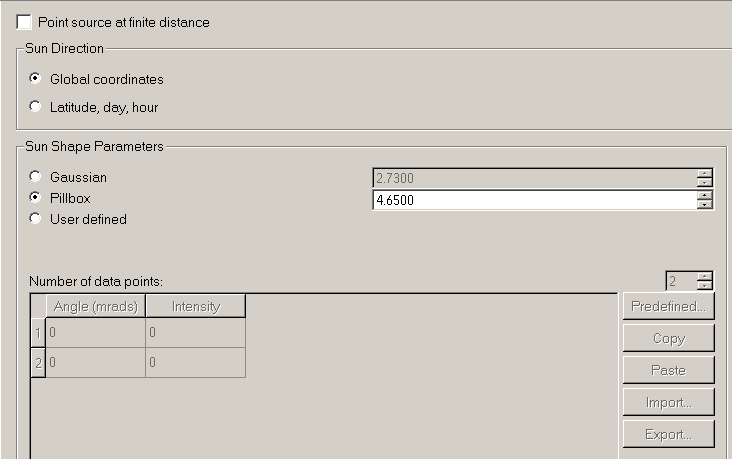
\includegraphics[width=0.5\textwidth]{figures/sunshape}\label{fig:forma}}
  \caption{\label{fig:soltrace} Del lado izquierdo se muestrea el indice del programa de SolTrace y del izquierdo las opciones para definir la forma solar.}
\end{figure}

\section{Propiedades ópticas}
\label{sec:opticas}

En un concentrador solar, varios factores estadísticos independientes contribuyen al error óptico: errores de pendiente\footnote{El error de pendiente engloba los errores macroscópicos.}, ausencia de la especularidad ideal, errores de seguimiento, deformaciones y desplazamientos del receptor.

Se considera generalmente que los errores pueden ser representados adecuadamente por distribuciones de probabilidad Gaussiana \citep{Pettit1977characterization}. El error global es una combinación de los diferentes errores y su dispersión estándar es una combinación en cuadratura de los errores individuales, Ec.\ref{eq:errores}.

\begin{equation}
  \label{eq:errores}
  \sigma_{\text{\'optica}}^2 = \sigma_{\text{especular}}^2 + 4\sigma_{\text{pendiente}}^2 + \sigma_{\text{seguimiento}}^2
\end{equation}
$\sigma_{\text{pendiente}}$ es multiplocado por 2 debido a la ley de Snell; en reflectores Fresnel $\sigma_{\text{seguimiento}}$ debe ser también multiplicada por 2.

El ancho total del rayo $\sigma_{\text{total}}$ es obtenida al agregar el semi-ángulo del disco solar.

\begin{equation}
  \label{eq:total}
  \sigma_{\text{total}}^2 = \sigma_{\text{\'optica}}^2 + \sigma_{\text{sol}}^2
\end{equation}

En la sección de propiedades ópticas (\emph{Optical Properties}) del índice principal del programa podemos definir las propiedades ópticas de nuestros materiales a utilizar.

\begin{itemize}[noitemsep]
\item Reflectancia
\item Transmitancia
\item Error de pendiente
\item Error especular
\item Tipo de error
\end{itemize}

\begin{figure}[h!]
  \centering
  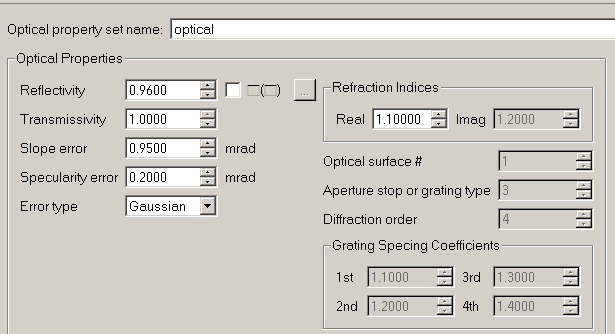
\includegraphics[width=0.7\textwidth]{figures/optica}
  \caption{\label{fig:optica} Propiedades ópticas.}
\end{figure}

Las propiedades ópticas dependerán del material del concentrador y del receptor que estemos utilizando.

\section{Etapas del trazado de rayos}
\label{sec:etapas}

Es en esta sección donde podemos definir las características de nuestro concentrador y del receptor. Es posible definir más de una etapa, pero estas etapas deben de ser subsecuentes. En la sección de etapas podemos distingir tres apartados. El primero de ellos es \emph{Stage Properties} en donde podemos asignar un nombre a la etapa y en donde esta seleccionada la etapa \emph{Multiple hits per ray} que nos indica que en esa etapa el rayo puede incidir varias veces; la opción \emph{Virtual stage} es utilizada cuando se desea saber que esta ocurriendo en una intervalo ente el concentrador y el receptor pero sin afectar la trayectoria de los rayos. Otra sección es \emph{Global Coordinates}, puede ser utilizada para generar sistemas de referencia locales. En sección de \emph{Element Editing} podemos definir los elementos que estrán interactuando en el trazado de rayos, condentradores o receptores.

\begin{itemize}[noitemsep]
\item \emph{Insert}. Puedes incentar elementos necesarios para la simulación
\item \emph{Append}. Te permite agregar elementos
\item \emph{Delete}. Como su nombre lo indica, puedes eliminar elementos
\end{itemize}

Una vez que agregas los elementos deseados pudes ir modificando las propiedades de cada uno de ellos. Indicando su posición ($x$, $y$, $z$), su \emph{Aimpoint} (ver \ref{subsec:aimpoint}), la apertura, el tipo de superficie, la intereacción del elemento y sus propiedades ópticas.

\begin{figure}[h!]
  \centering
  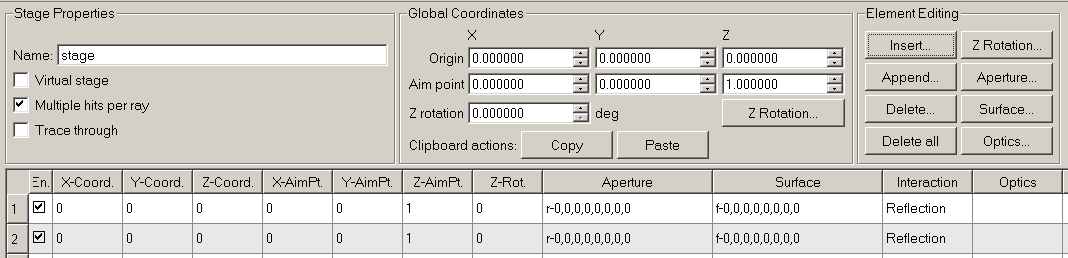
\includegraphics[width=1.0\textwidth]{figures/stage}
  \caption{\label{fig:etapa} Característica de las etapas.}
\end{figure}

Los tipos de aperturas y superficies que pueden ser utilizadas, se muestran en la Figura~\ref{fig:elementos}. A las cuales podemos ingresar al seleccionar el botón de \emph{Aperture} o \emph{Surface}, respectivamente.

\begin{figure}[ht]
  \centering
  \subfigure[]{
    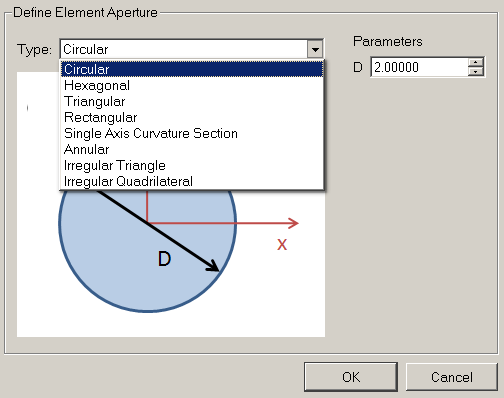
\includegraphics[width=0.45\textwidth]{figures/apertura}}
  \subfigure[]{
    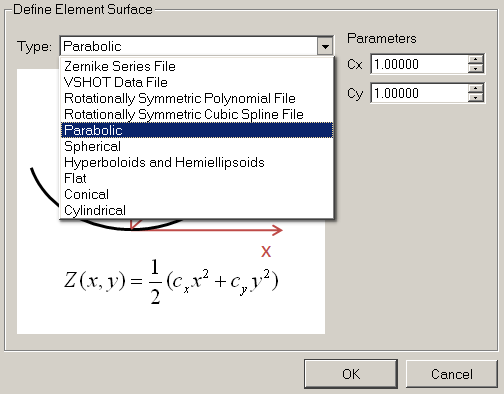
\includegraphics[width=0.455\textwidth]{figures/superficie}}
  \caption{\label{fig:elementos} Tipos de apertura,a la izquierda, y de superficie, a la derecha.}
\end{figure}

\subsection{Aimpoint}
\label{subsec:aimpoint}

El \emph{aimpoint} es un vector que define SolTraces y nos indica la orientación de una superficie. Considerese la Figura~\ref{fig:aimpoint} en donde se muestra una superficie plana en donde incide el vetor solar $\hat s$ el cual es reflejado con una dirección $\hat r$ que incide en el objetivo deseado; se definen adicionalmente los vectores $\vec R_F$ y $\vec R_T$ que son los vectores que van desde el origen de las coordenadas globales a la superficies y al objetivo, respectivamente. La orientación de dicha superficie esta definida por su \emph{aimpoint} que es un vector que va desde el origen a cualquier punto del vector normal $\hat n$ de la superficie. El \emph{aimpoint} es la suma de los vectores $\vec R_F$ y $\vec n$. Hay que hacer notar que si nuestra superficie esta en el origen el \emph{aimpoint} coincidirá con la  dirección del vector normal, dado que $\vec R_F$ es cero. Pero para las demás superficies que se encuentran fuera del origen el $\vec R_F$ es diferente de cero. Como lo muestra la Figura~\ref{fig:aimpoint} el \emph{aimpoint} de una superficie fuera del origen esta dado por la Ec.~\ref{ec:aimpoint}

\begin{equation} \label{ec:n}
  \hat n = \dfrac{\hat s + \hat r}{\Vert \hat s + \hat r \Vert}
\end{equation}

\begin{equation} \label{ec:aimpoint}
  \vec a = \vec R_F + \hat n 
\end{equation}



\begin{figure}[h!]
  \centering
  \subfigure[]{
    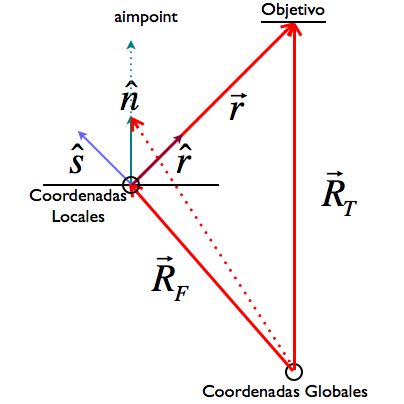
\includegraphics[width=0.45\textwidth]{figures/aimpoint01}\label{fig:base}}
  \subfigure[]{
    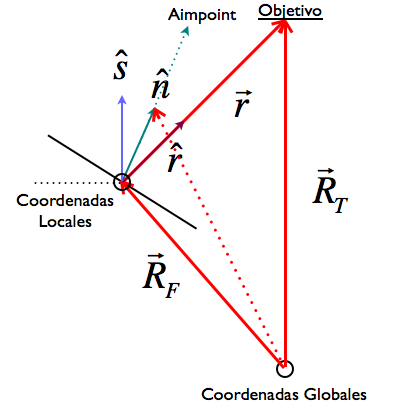
\includegraphics[width=0.45\textwidth]{figures/aimpoint02}\label{fig:igAim}}
  \caption{\label{fig:aimpoint} Definición de \emph{aimpoint}.}
\end{figure}


\section{Trazado de rayos}
\label{sec:trazado}

Una vez que se han definido las diferentes secciones de los elementos se procede a realizar la simulación de trazado de rayos, para lo cual es necesario indicar el número de rayos para la interacción, hay que recordar que SolTrace utiliza el método de Monte Carlo, y dado que se trata de un método estadístico, entre más rayos se utilicen el resultado obtenido será más preciso. Usualmente se selecciona un número de rayos pequeño, e.g., un millón es un buen número para iniciar, y corregir tus posibles errores, sin embargo es necesario realizar un analísis de independencia de malla para conocer el número óptimo de rayos necesarios para nuestra simulación.

\begin{figure}[h!]
  \centering
  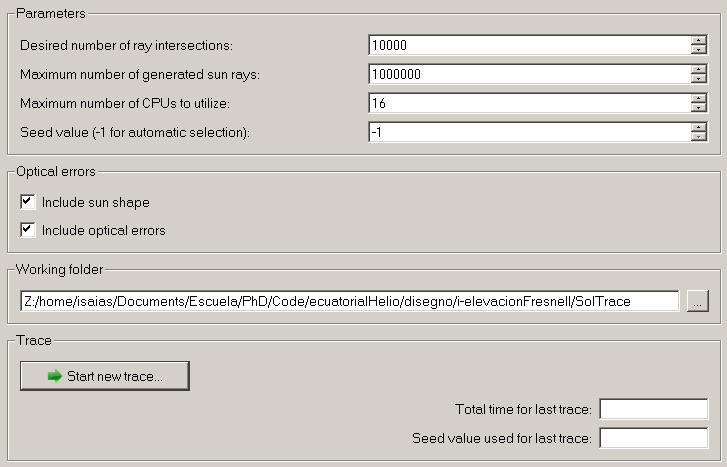
\includegraphics[width=0.7\textwidth]{figures/raytrace}
  \caption{\label{fig:trazado} Opciones de trazado de rayos.}
\end{figure}

\section{Plato parabólico}
\label{sec:plato}

\begin{problem}
Simule un plato parabólico en SolTrace que tenga un ángulo de borde $\psi_b = \pi/2$ y una apertura de dos metros.  
\end{problem}



\TheSolution Primero, considerese la parábola de la Figura~\ref{fig:parabola} generada con la con la ecuación~\eqref{eq:parabola} definida por el foco $f$.

\begin{equation}
  \label{eq:parabola}
  y = \dfrac{x^2}{4f} -f
\end{equation}


\begin{figure}[ht]
  \centering
  \subfigure[]{
    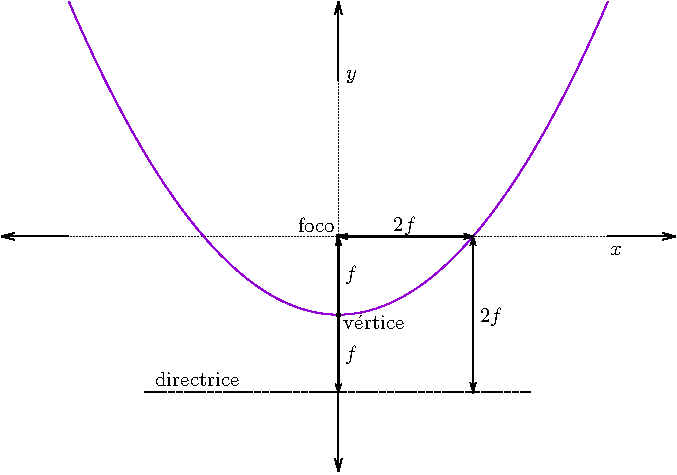
\includegraphics[width=0.45\textwidth]{figures/parabola}}
  \subfigure[]{
    \includegraphics[width=0.45\textwidth]{figures/parabolaPolares}}
  \caption{\label{fig:parabola} Parábola con el foco en el origen.}
\end{figure}

Es decir, que si el ángulo de borde es de $\pi/2$, implica que $x_b=1$~m ya que la apertura es de dos metros y entonces $f$ es de 0.5~m.

Sabemos\cite{Rabl1985active} que para un receptor cilíndrico el diámetro del receptor esta dado por la ecuación~\eqref{eq:diametro}. Si consideramos que el semi-ángulo de aceptación $\Delta_r$ es del tamaño del cono solar, entonces $\Delta = $4.65~mrad. Luego entonces podemos calcular el diámetro del receptor ideal y es igual 9.3~mm.



\begin{equation}
  \label{eq:diametro}
  D = \dfrac{4 \Delta_r f}{1 + \cos \psi_b}
\end{equation}

\ASolution Para simular este disco parábolico consideraremos un vector solar paralelo al eje $z$, es decir $\hat s = (0, 0, 1)$ y una forma Gaussiana. Respecto a los paramámetros ópticos, para el concentrador consideraremos una reflectividad casi especular de 0.96, una transmitancia de practicamente cero, sin errores de pendiente y especularidad. La Tabla~\ref{tab:opticaDisco} muestra los parámetros mencionados. Para el receptor generamos otro elemento en donde la reflectancia será nula.

\begin{table}[h]
  \centering
  \begin{tabular}[h]{ccccc}
    \toprule
    Reflectivity & Transmissivity & Slope error & Specularity error & Error type\\
    \midrule
    0.96         & 0.0001         & 0.0001      & 0.0001            & Gaussian\\
    \bottomrule
  \end{tabular}
  \caption{\label{tab:opticaDisco} Propiedades ópticas}
\end{table}

En la sección de etapas vamos agenerar nuevamente dos elementos, una para el concentrador y una para el receptor. La Tabla~\ref{tab:etapaReceptorD} muestra los parámetros del concentrador, para lo cual es necesario primero, mediante el boton \emph{Insert}, insertar un elemento. En el cual ingresaremos la posición del paraboloide, que sera el origen, en donde la su normal coincide con el \emph{aimpoint} es decir $(0, 0, 1)$. La apertura es circular con un diámetro de 2~m y el tipo de superficie es una parabóla con un foco de $f = 0.5$~m. El tipo de interacción es \emph{Reflection} y en el elemento \emph{Optics} seleccionamos el de \emph{concentrador} que previamente habíamos definido.

\begin{table}[h]
  \centering
  \scriptsize
  \begin{tabular}[h]{lllllllll}
    \toprule
    X-C & Y-C & Z-C & X-AimP & Y-AimP & Z-AimP & Z-Rot & Aperture & Surface\\
    \midrule
    0 & 0 & 0 & 0 & 0 & 1 & 0 & c-2,0,0,0,0,0,0,0 & p-1,1,0,0,0,0,0,0\\
    \bottomrule
  \end{tabular}
  \caption{\label{tab:etapaReceptorD} Etapa del concentrador.}
\end{table}

En la segunda etapa generamos el receptor circular plano posicionado en el foco, es decir, úbucado en $(0, 0, 0.5)$, y con un \emph{aimpoint} de $(0, 0, -1)$ sigue siendo paralelo al eje $z$ pero en sentido contrario. Seguimos teniendo una apertura circular con el radio calculado de 9.3~mm, pero ahora tenemos una superficie plana. Ahora las propiedades ópticas seran las definidas como \emph{concentrador}.

\begin{table}[h]
  \centering
  \scriptsize
  \begin{tabular}[h]{lllllllll}
    \toprule
    X-C & Y-C & Z-C & X-AimP & Y-AimP & Z-AimP & Z-Rot & Aperture & Surface\\
    \midrule
    0 & 0 & 0.5 & 0 & 0 & -1 & 0 & c-0.0093,0,0,0,0,0,0,0 & f-0,0,0,0,0,0,0,0\\
    \bottomrule
  \end{tabular}
  \caption{\label{tab:etapaReceptorR} Etapa del receptor }
\end{table}

Ya que tenemos de finido el sistema podemos proceder a realizar la simulación, para lo cual seleccionaremos 1,000,000 de rayos. Una vez indicado el numero de rayos procedemos a realizar la simulación mediante el botón \emph{Start new trace}.

La sección de \textbf{Results} tiene tres secciones: \emph{Intersections}, \emph{Flux Maps} y \emph{Ray Data}. En la sección de \emph{Intersections} podemos visualizar los distintos elementos simulados, en donde solo observaremos la interacción de los rayos con las superficies si existen, también tenemos la opción de imprimir la trayectoria de los rayos deseados.

La Figura~\ref{fig:inter} muestra la sección de \emph{Intersections} en ella podemos seleccionar la etapa de trazados de rayos y los elementos que contienen para visualizarlos. Una vez seleccionados se visualizan en la interacción de los rayos con las superficies que interactual, a demás si seleccionamos \emph{Plot path of ray \#s} podemos indicar el intervalo de rayos que deseamos visualizar. Los rayos que se muestran en color rojos son aquellos que no inciden en el receptor. En esta sección se indica cual es la irradiancia considerada para la simulación, en este caso es de 1,000 $\rm W/m^2$. Por ultimo se muestra una sección  con un resumen de la información del trazado de rayos.

\begin{figure}[ht]
  \centering
  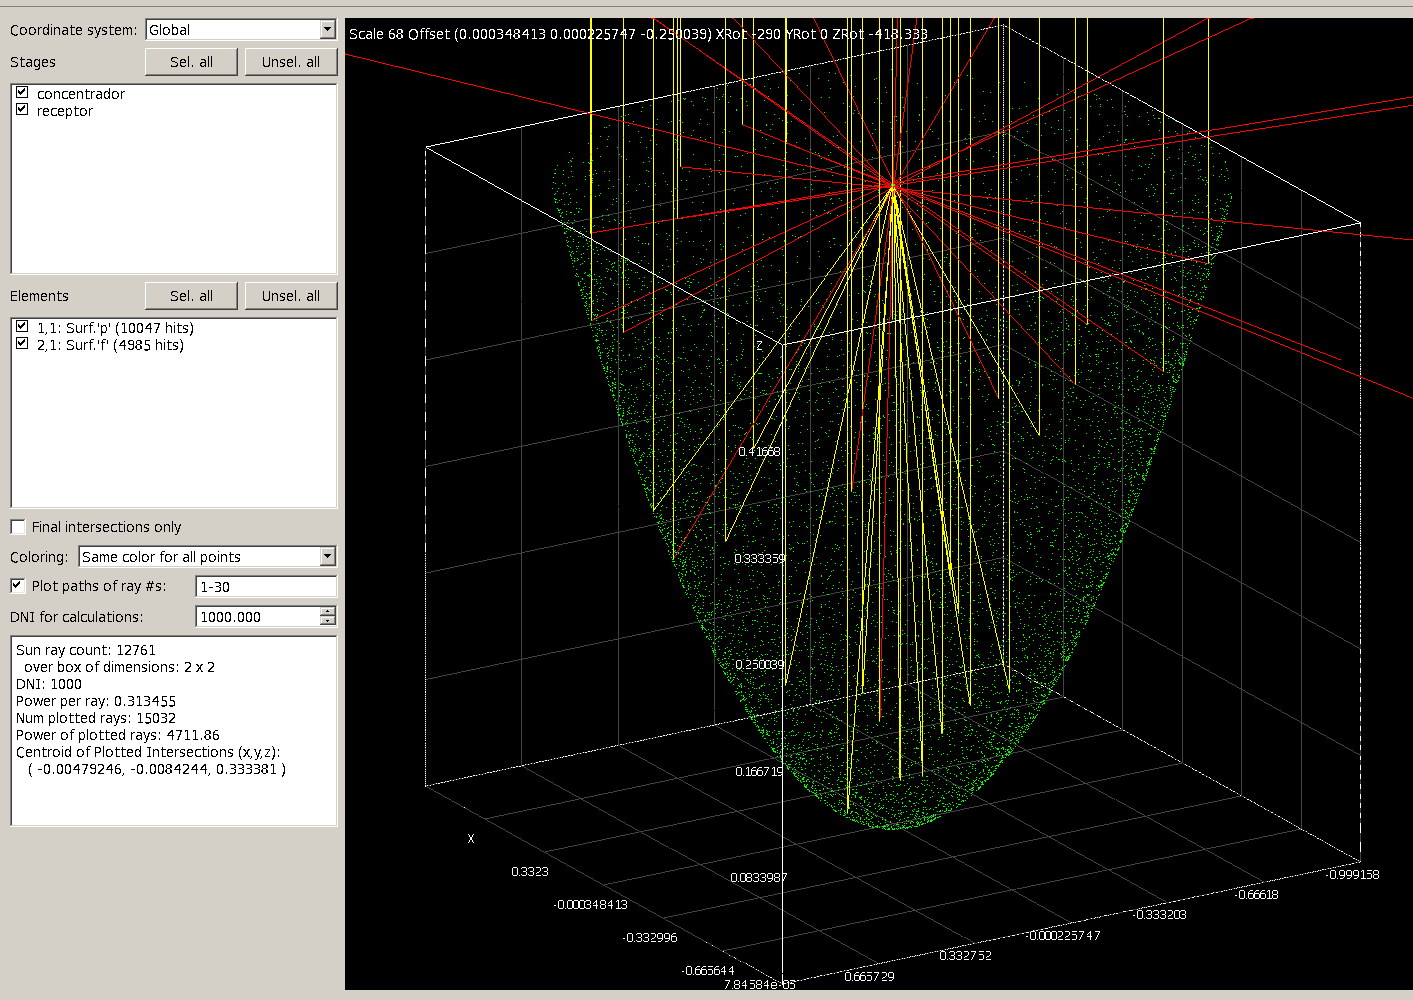
\includegraphics[width=1.0\textwidth]{figures/intersecciones}
  \caption{\label{fig:inter}  Sección de \emph{Intersections} de resultados en SolTrace.}
\end{figure}


En la sección de \emph{Flux Maps} se puede seleccionar la sección de interes a visualizar. En este casao unicamente tenemos un elemento. En esta sección podemos indicar el tamaño de la malla, que por default es de 20$\times$20. Existe también una sección para exportar los datos que nos genera dos archivos uno de con la extensión de ``.tec'' y ``.flx'', el primero se un archivo de datos que contiene la coordenadas y el valor de intensidad que le corresponde. El segundo archivo es la misma información pero en un arreglo matricial. Y por último, existe una sección en donde se muestran un resumen de la simulación. La Figura~\ref{fig:flux} muestra la pestaña de \emph{Contour Plot} en donde se observa la distribución de flujo, la pestaña de \emph{Surface Plot} nos muestra la misma información en 3D.

\begin{figure}[ht]
  \centering
  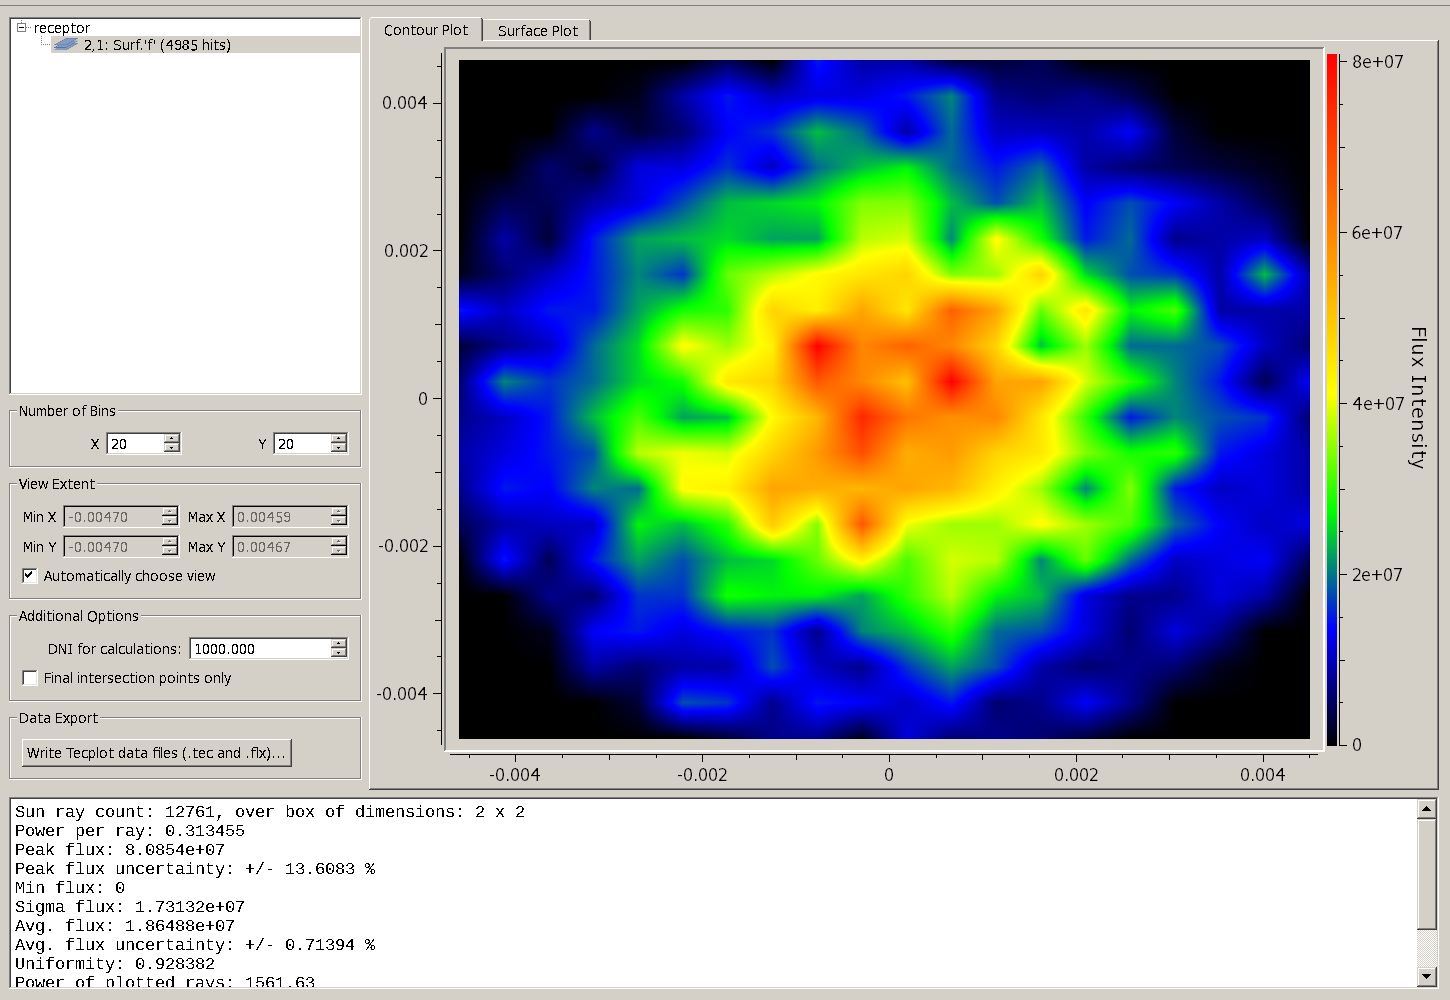
\includegraphics[width=1.0\textwidth]{figures/flux}
  \caption{\label{fig:flux} Distribución de flujo en el receptor.}
\end{figure}

La sección de \emph{Ray Data} nos permite explortar la información del trazado de rayos en un archivo ``.csv''.

Por último realizaremos un trazado de rayos con 7 millones de rayos, mismo que exportaremos con una malla de 35$\times$35.

\begin{figure}[ht]
  \centering
  \subfigure[]{
    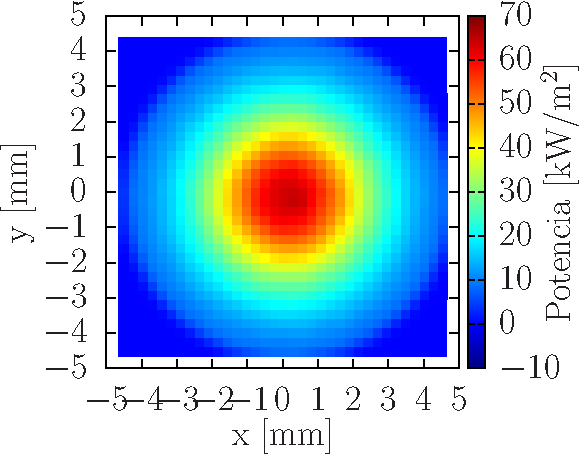
\includegraphics[width=0.45\textwidth]{figures/flux_disco}}
  \subfigure[]{
  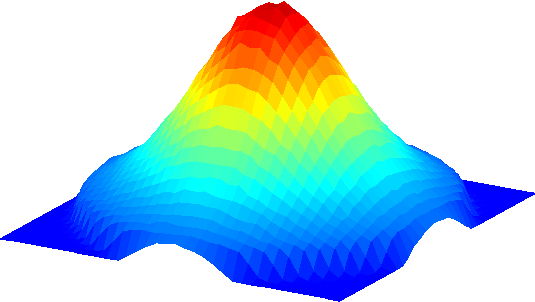
\includegraphics[width=0.5\textwidth]{figures/receptor3d}}
  \caption{\label{fig:fluxDisco} Flujo en el receptor.}
\end{figure}



%%% Local Variables: ***
%%% mode: latex ***
%%% TeX-master: "taller.tex" ***
%%% End: ***

\section{Canal Parabólico}
\label{sec:canal}

\begin{problem}
  Realice una el trazados de rayos de un canal parabólico que tiene un ángulo de borde $\psi = 80^\circ$, y un ancho de apertura de 1.5~m.
\end{problem}

\TheSolution Sabemos que de la ecuación~\ref{eq:rhof} podemos calcular el foco $f$ de la parabóla, dado que conocemos el ángulo de borde $\psi = 80^\circ$ y sabemos que $x_b = \rho \sin \psi_b$ en donde $x_b= 0.75$, debido a que la apertura es de 1.5~m. Calculamos $\rho$ que es igual a 0.76~m. Considerese la Figura~\ref{fig:canal}.

\begin{figure}[ht]
  \centering
  \includegraphics[width=1.0\textwidth]{figures/canalP}
  \caption{\label{fig:canal} Parabóla del concentrador de canal parabólico.}
\end{figure}

\begin{equation}
  \label{eq:rhof}
  \rho = \dfrac{2 f}{1 + \cos \psi_b}
\end{equation}
despejando $f$ y sustituyendo los valores correspondientes $f = 0.4469$~m.

Por otro lado, sabemos que el área de apertura es $A_p = (2 x_b) L$, por lo que podemos considerar una $L= 3$~m. Para el calculo del receptor utilizamos la ecuación~\ref{eq:diametro2}, nuevamente, en donde consideraremes el semi-ángulo de aceptación $\Delta = 4.65\rm mrad$ igual al tamaño del cono solar.

\begin{equation}
  \label{eq:diametro2}
  D = \dfrac{4 \Delta_r f}{1 + \cos \psi_b}
\end{equation}
sustituyendo los valores podemos calcular que el díametro ideal del receptor que es igual a 7.08~mm.

\ASolution Para la simulación de trazado de rayos utilizamos utilizamos un vector solar $\hat s = (0,0,1)$, una función \emph{Pillbox} forma solar. Las propiedades ópticas del concentrador se muestran en la Tabla~\ref{tab:opticaCanal}


\begin{table}[h]
  \centering
  \begin{tabular}[h]{ccccc}
    \toprule
    Reflectivity & Transmissivity & Slope error & Specularity error & Error type\\
    \midrule
    0.96         & 0.0001         & 0.0001      & 0.0001            & Gaussian\\
    \bottomrule
  \end{tabular}
  \caption{\label{tab:opticaCanal} Propiedades ópticas}
\end{table}

Se generan dos etapas una para el concentrador y otra para el receptor. Para simular un canal parabólico se selecciona la apertura \emph{Rectangular} y se considera una longitud de 3~m. Se utiliza una superficie parabólica con el foco calculado. La interacción es de reflexión y los parámetros ópticos los definidos con anterioridad.

\begin{table}[h]
  \centering
  \scriptsize
  \begin{tabular}[h]{lllllllll}
    \toprule
    X-C & Y-C & Z-C & X-AimP & Y-AimP & Z-AimP & Z-Rot & Aperture & Surface\\
    \midrule
    0 & 0 & 0 & 0 & 0 & 1 & 0 & r--0.75,3,0,0,0,0,0,0 & p-1.1213,0,0,0,0,0,0,0\\
    \bottomrule
  \end{tabular}
  \caption{\label{tab:etapaReceptorD} Etapa del concentrador.}
\end{table}

Las propiedades del receptor se muestran en la Tabla~\ref{tab:etapaRecC}, donde el receptor lo colocamos en el foco. La apertura también es del tipo \emph{Single Axis Curvature Section} con una longitud de 3~m. La superficie es de tipo cilindrico con el díamero calculado.
\begin{table}[h]
  \centering
  \scriptsize
  \begin{tabular}[h]{lllllllll}
    \toprule
    X-C & Y-C & Z-C & X-AimP & Y-AimP & Z-AimP & Z-Rot & Aperture & Surface\\
    \midrule
    0 & 0 & 0.4469 & 0 & 0 & -1 & 0 & l-0,0,3,0,0,0,0,0 & t-282.486,0,0,0,0,0,0,0\\
    \bottomrule
  \end{tabular}
  \caption{\label{tab:etapaRecC} Etapa del receptor }
\end{table}

Realizando un simulación para con un millón de rayos se obtienen los resultados mostrados en la Figura~\ref{fig:canal}.

\begin{figure}[ht]
  \centering
  \subfigure[]{
    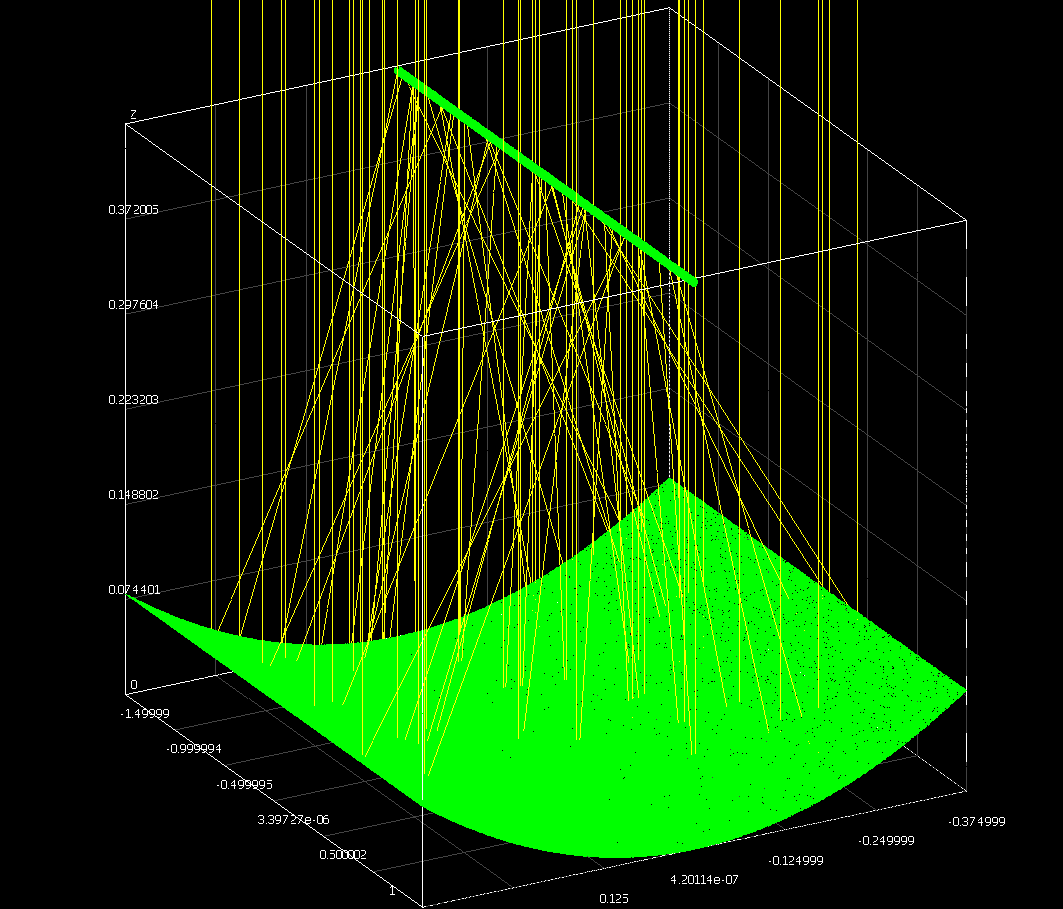
\includegraphics[width=0.41\textwidth]{figures/canal}}
  \subfigure[]{
    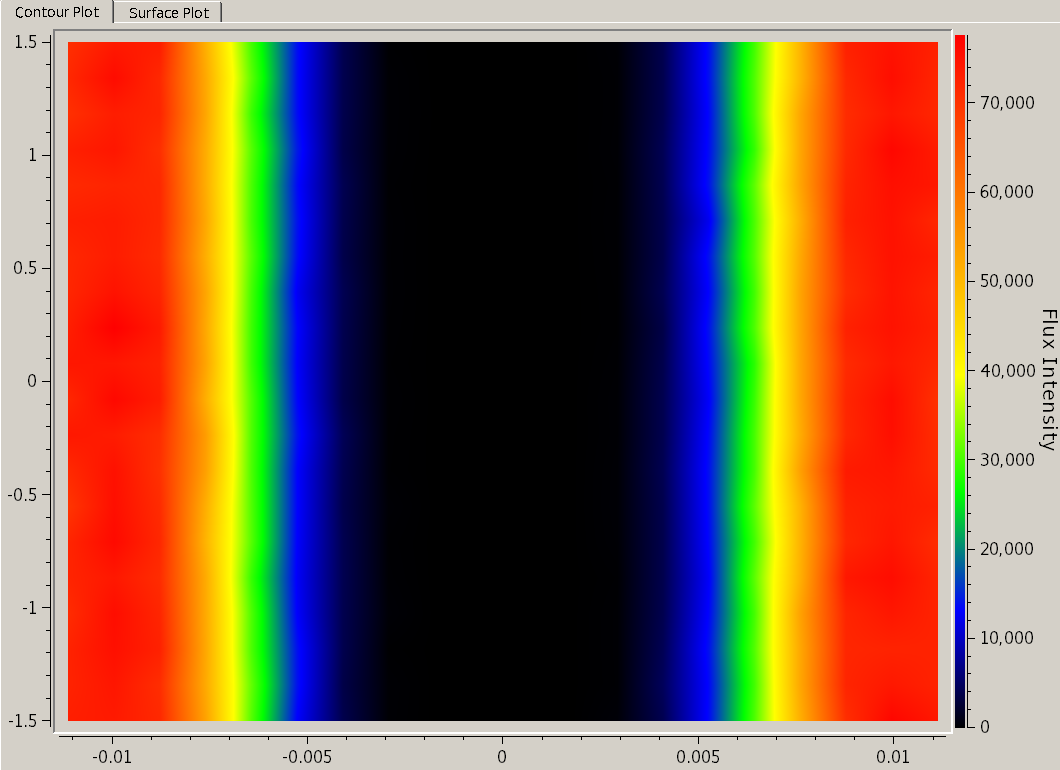
\includegraphics[width=0.48\textwidth]{figures/fluxCanal}}
  \caption{\label{fig:canal} Trazado de rayos del un canal parabólico.}
\end{figure}

%%% Local Variables: ***
%%% mode: latex ***
%%% TeX-master: "taller.tex" ***
%%% End: ***

\section{Helióstato}
\label{sec:helio}

\begin{problem}
  Realizar el trazado de rayos de un helióstato y un receptor colocado en lo alto de una torre, ver Figura~\ref{fig:helio}. Consideré que el helióstato tiene unas dimensiones de 1$\times$1~m, y se encuentra a 50~m de la torre, hacia el norte. El receptor esta a una altura de 32~m. Considere que el vector solar es igual a $\hat s = (0, 0, 1)$.
\end{problem}

\begin{figure}[ht]
  \centering
  \includegraphics[width=1.0\textwidth]{figures/helio}
  \caption{\label{fig:helio} Heliostato}
\end{figure}


\TheSolution Sabemos que por la ley de reflección podemos calcular la dirección de la normal $\hat n$ del helióstato con la ecuación~\ref{eq:nst}, de donde conocemos $\hat s$ y el vector de reflexión es $\vec R = T - H$ y su valor unitario es de $\hat r = (0.00, -0.8422, 0.5390)$. Por lo que el valor de $\hat n = (0.00, -0.480, 0.877)$.

\begin{equation}
  \label{eq:nst}
  \hat n = \dfrac{\hat s + \hat r}{\| \hat s + \hat r \|}
\end{equation}

El valor del \emph{aimpoint} $\vec A = \vec R_F + \hat n$, donde $\\vec R_F$ es un vector que va del origen a la posición del helióstato, en este caso $\vec R_F = (0, 50, 0)$, y $\vec A = (0, 49.52, 0.877)$.

\ASolution:

Considerese las propiedades ópticas de la Tabla~\ref{tab:opticaHelio} para el helióstato.

\begin{table}[h]
  \centering
  \begin{tabular}[h]{ccccc}
    \toprule
    Reflectivity & Transmissivity & Slope error & Specularity error & Error type\\
    \midrule
    0.95         & 0.0001         & 2.500      & 0.2000            & Gaussian\\
    \bottomrule
  \end{tabular}
  \caption{\label{tab:opticaHelio} Propiedades ópticas}
\end{table}

Nuevamente se requieren dos etapas, una para el helióstato y otra para el receptor. La posición del helióstato es $H = (0, 50, 0)$, y su \emph{aimpoint} es el calculado. El Helióstato tiene una apertura de 1$\times$1~m y en este caso se trata de una superficie plana. La Tabla~\ref{tab:etapaHelioC} indica los parámetros indicados.

\begin{table}[h]
  \centering
  \scriptsize
  \begin{tabular}[h]{lllllllll}
    \toprule
    X-C & Y-C & Z-C & X-AimP & Y-AimP & Z-AimP & Z-Rot & Aperture & Surface\\
    \midrule
    0 & 50 & 0 & 49.52 & 0.877 & 0 & 0 & r-1,1,0,0,0,0,0,0 & p-0,0,0,0,0,0,0,0\\
    \bottomrule
  \end{tabular}
  \caption{\label{tab:etapaHelioC} Etapa del concentrador.}
\end{table}

El receptor, en este caso, se trata de una superficie plana orientada hacia el norte. Dado que no indican el tamaño utilizaremos un receptor de 3$\times$3~m, como lo indica la Tabla~\ref{tab:etapaHelioR}.

\begin{table}[h]
  \centering
  \scriptsize
  \begin{tabular}[h]{lllllllll}
    \toprule
    X-C & Y-C & Z-C & X-AimP & Y-AimP & Z-AimP & Z-Rot & Aperture & Surface\\
    \midrule
    0 & 0 & 32 & 0 & 1 & 32 & 0 & r-3,3,0,0,0,0,0,0 & f-0,0,0,0,0,0,0,0\\
    \bottomrule
  \end{tabular}
  \caption{\label{tab:etapaHelioR} Etapa del receptor }
\end{table}

Posteriormente se realiza una simulación considerando a millón de rayos. La Figura~\ref{fig:rayHelio} muestra la simulación.

\begin{figure}[ht]
  \centering
  \subfigure[]{
    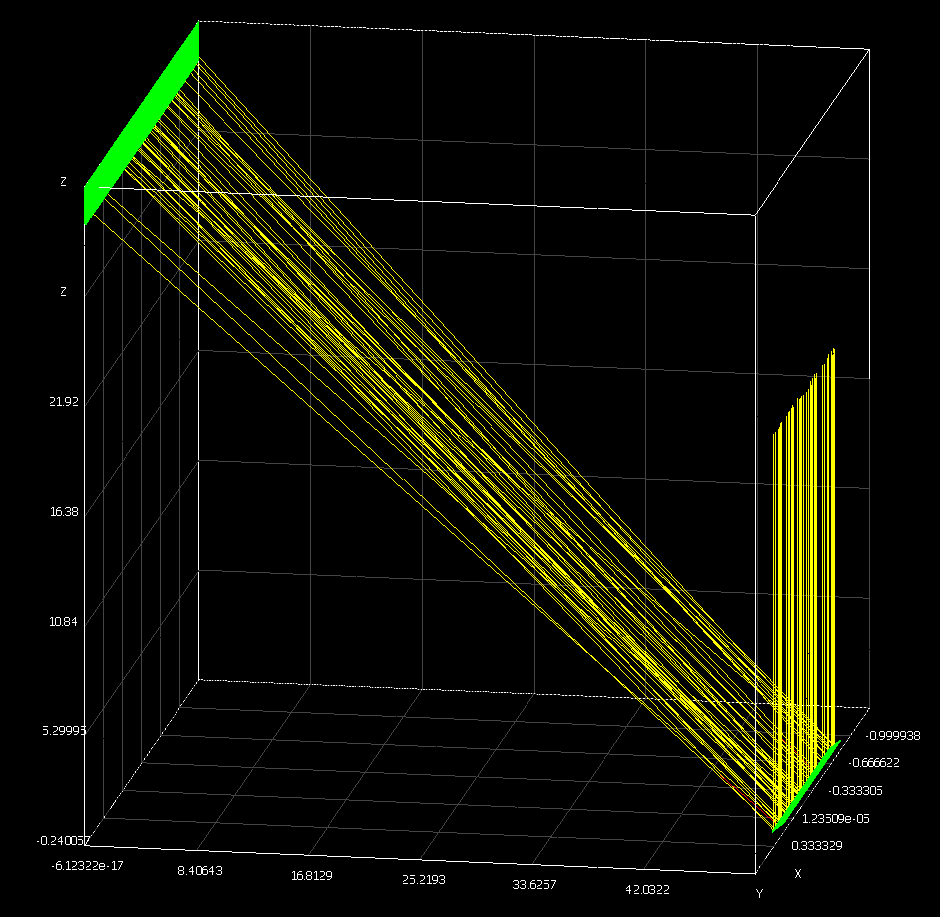
\includegraphics[width=0.33\textwidth]{figures/rayHelio}}
  \subfigure[]{
    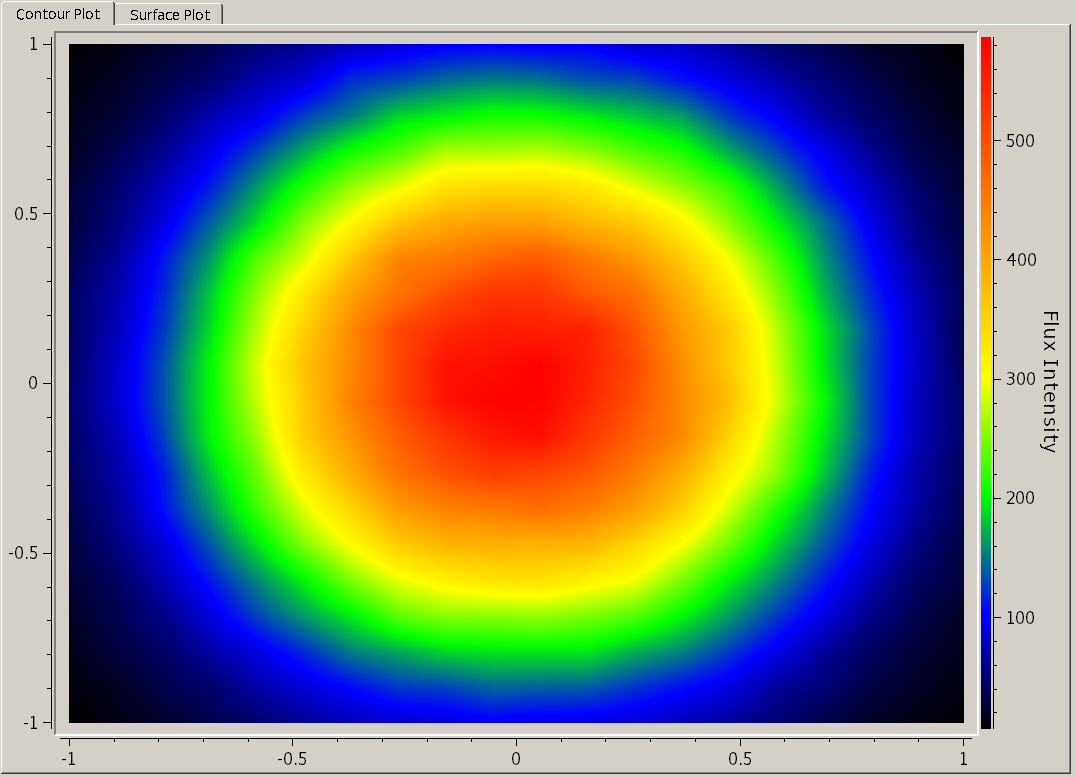
\includegraphics[width=0.45\textwidth]{figures/fluxHelio}}
  \caption{\label{fig:rayHelio} Simulación de trazado de rayos de un helióstato.}
\end{figure}



%%% Local Variables: ***
%%% mode: latex ***
%%% TeX-master: "taller.tex" ***
%%% End: ***

\section{Scripting}
\label{sec:script}

En SolTrace se pude utilizar scripts, ver Figura~\ref{fig:script}, para programar el trazado de rayos mediante \href{https://github.com/NREL/lk}{LK}. De esta manera es posible hacer simulaciones en lo largo del tiempo.


\begin{figure}[ht]
  \centering
  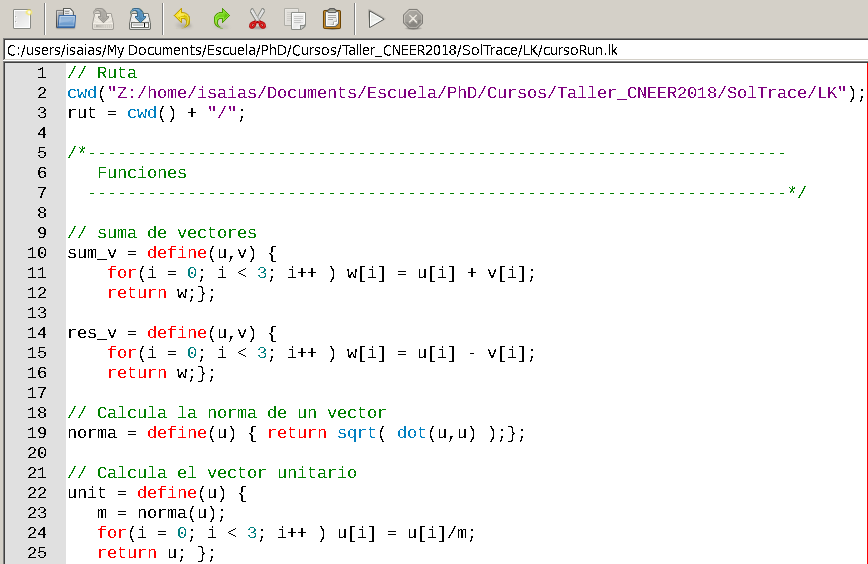
\includegraphics[width=1.0\textwidth]{figures/script}
  \caption{\label{fig:script} Script LK para la SolTrace.}
\end{figure}

El script LK es una modificación del lenguaje \verb=C=, puedes para conocer las característitcas básicas revisa el documento \href{https://github.com/NREL/lk/blob/develop/doc/lk_guide.pdf}{Guide LK}. A continuación se muestra un script para simular el helióstato del problema de la Sección~\ref{sec:helio}.


\lstinputlisting{./../LK/cursoRun.lk}

\section{Cálculo de la radiación solar}
\label{sec:radiacion}

Dado que el valor de la irradiancia varia con el tiempo, es necesario calcularla en el tiempo.


La radiación directa puede ser calculada, para diferentes horas y días, con un módelo de cielo claro~\citep{Dunham2013optical}, utilizando:

\begin{equation}
  \label{eq:DNI}
  G_b = G_0 \tau^{AM^{0.678}}
\end{equation}
donde $G_0$ es la constante solar de $1,367 \rm W/m^2$, y $\tau$ es la transmitancia atmosférica, que para condiciones de cielo claro tiene un valor de 0.7, y la masa de aire es obtenida como función de la altitud del lugar.
\begin{equation}
  \label{eq:AM}
  AM = \frac{ \exp(-0.0001184\,h_{\rm altitud})}{\cos \theta_z + 0.5057(96.080-\theta_z)^{-1.634}}
\end{equation}
$\theta_z$ es el ángulo cenital del vector solar, y $h_{\rm altitud}$ la altura sobre el nivel del mar.


%%% Local Variables: ***
%%% mode: latex ***
%%% TeX-master: "taller.tex" ***
%%% End: ***



\bibliographystyle{plain}
\bibliography{taller}

\end{document}
